\documentclass[10pt,utf8]{beamer}

\mode<presentation> {
%  \usetheme{Boadilla}
  \usetheme{Madrid}
%	\usetheme{Fzu}
  \setbeamercovered{transparent}
}

\usepackage{palatino}
\usepackage{graphicx}
\usepackage{array}
\usepackage{color}
\usepackage{subfigure}
\usepackage{colortbl}
\usepackage{amsmath}
\usepackage{hyperref}
\usepackage{listings}
\usepackage{fancyvrb}

\setbeamertemplate{caption}{\raggedright\insertcaption\par} %turn off caption prefix ("Figure")

\title{Sanlock troubleshooting}
\author{Vojtěch Juránek}
\institute[Red Hat]{oVirt storage team}
\date{1.~12.~2020, oVirt internal}

\lstdefinestyle{Bash}{
	basicstyle          = \large\ttfamily,
	language            = Bash,
	numbers             = left,
	numberstyle         = \small,
	stepnumber          = 1,
	numbersep           = 5pt,
	backgroundcolor     = \color{white},
	showspaces          = false,
	showstringspaces    = false,
	showtabs            = false,
	frame               = single,
	tabsize             = 2,
	captionpos          = b,
	breaklines          = true,
	breakatwhitespace   = false,
	morestring          = [b]",
	stringstyle         = \color{blue},
	keywordstyle        = \color{magenta},
	commentstyle        = \color{gray},
	identifierstyle     = \color{black},
	moredelim           = **[is][\bfseries]{`}{`},
	moredelim           = **[is][\color{magenta}]{!}{!}, 
	fancyvrb            = true,
}


\begin{document}

\begin{frame}
    \titlepage
\end{frame}

\begin{frame}
  \frametitle{Storage virtualization}
  \begin{figure}
    \centering
    
\includegraphics[height=5cm]{./img/virt-storage.eps}
    \caption{\tiny{Source: \url{https://sharedstorage.wordpress.com/2017/01/03/storage-virtualization/}}}
  \end{figure}
\end{frame}

\begin{frame}
  \frametitle{Data consistency}
  \begin{figure}
    \centering
    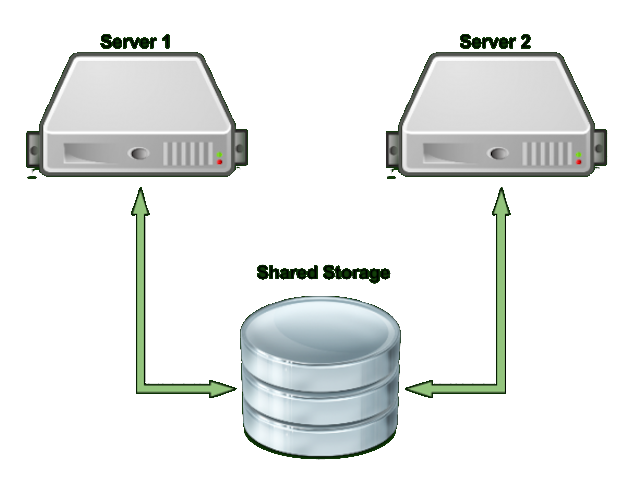
\includegraphics[height=5cm]{./img/disk-paxos.eps}
    \caption{\tiny{Source: \url{https://www.linuxjournal.com/content/high-availability-storage-ha-lvm}}}
 \end{figure}
\end{frame}

\begin{frame}
  \frametitle{sanlock}
  \begin{itemize}
    \item $\Delta$-leases 
    \item Paxos leases
    \item Watchdog
  \end{itemize}
\end{frame}

\begin{frame}
  \frametitle{sanlock: big picture}
  \begin{itemize}
    \item $\Delta$-leases are used for acquiring/confirming unique ID for each host (only for sanlock internal usage)
    \item Paxos leases are used for acquiring locks for resources (meaning of the lock is determined by the application).
    \item Unique host IDs are use for Paxos leases for mapping host to its disk segment.
  \end{itemize}
\end{frame}

\begin{frame}
    \frametitle{sanlock: $\Delta$-Leases}
  \begin{itemize}
    \item In sanlock terminology called \textit{lockspaces}.
    \item Prevents two hosts to have same ID.
    \item Maximum number of hosts is 2000.
    \item Lockspace size is 1~MB (for block size 512B).
    \item Use options \texttt{-A} and \texttt{-Z} to change alignment and block size.
  \end{itemize}
\end{frame}

\begin{frame}
  \frametitle{sanlock: $\Delta$-Leases}
  \begin{itemize}
    \item sanlock renews $\Delta$-leases every 20 seconds by writing a new time stamp into appropriate $\Delta$-lease block.
    \item Lease renewal is used also for checking if host is alive.
  \end{itemize}
\end{frame}

\begin{frame}
  \frametitle{sanlock: Paxos leases}
  \begin{itemize}
    \item Fast to acquire.
    \item In sanlock terminology called \textit{resources}.
    \item Lease is acquired by the winner by writing its ballot into to the first block of the resource disk area.
    \item sanlock uses $\Delta$-lease renewals also for Paxos leases renewal in given lockspace.
  \end{itemize}
\end{frame}

% \begin{frame}
%   \frametitle{sanlock: Paxos leases}
%   \begin{itemize}
%     \item Host IDs are used as Paxos leases owners.
%     \item Size of Paxos lease is also 1~MB (for block size 512B).
%     \item Lease is acquired by the winner by writing its ballot into to the first block of the resource disk area.
%   \end{itemize}
% \end{frame}

\begin{frame}
    \frametitle{Resources}
    \begin{itemize}
    \item \small \color{blue}\url{https://pagure.io/sanlock}\color{black}
     \item \color{blue}\href{http://lamport.azurewebsites.net/pubs/disk-paxos-disc.pdf}{E. Gafni, L. Lamport, Disk Paxos}\color{black}
     \item \color{blue}\href{https://groups.csail.mit.edu/tds/papers/Chockler/TR934.ps}{G. Chockler, D. Malkhi, Light-Weight Leases for Storage-Centric Coordination}\color{black}
    \end{itemize}
\end{frame}

\begin{frame}
    \frametitle{Questions?}
    \centering
     \textbf{\Huge{Thank you!}}
    
    \vspace{1.5cm}
    
    \textbf{\Huge{Questions?}}
\end{frame}

\end{document}
